\section{Thiết kế kiến trúc và công nghệ}
\label{sec:architecture}

\subsection{Phạm vi và hướng tổ chức}

BrewLite sử dụng kiến trúc phân lớp trong một monorepo: ứng dụng web Next.js gọi REST API NestJS; backend truy cập PostgreSQL thông qua Prisma. Đây là kiến trúc của Bài tập lớn 1, phục vụ luồng xem menu, chọn size/topping, giỏ hàng, đăng nhập, đặt đơn, thanh toán mô phỏng và tra cứu đơn. Các cơ chế trạng thái đơn, chống thanh toán lặp, giữ tồn kho và khuyến mãi/điểm thưởng là phần hiện thực nghiệp vụ Task 10 của cùng đề bài; việc đạt toàn bộ tiêu chí chấp nhận cần được xác nhận bằng kết quả kiểm thử.

Backend được tổ chức thành một ứng dụng theo module, không tách thành các microservice. Cách tổ chức này cho phép một transaction bao trùm đơn hàng, tồn kho và điểm thưởng trong cùng CSDL, đồng thời giữ việc chạy thử bằng Docker Compose đơn giản. Các sơ đồ dưới đây thể hiện cấu trúc đã có trong mã nguồn; phần mở rộng được ghi rõ để tránh nhầm với phạm vi MVP.

\begin{figure}[htbp]
\centering
\begin{tikzpicture}[
  box/.style={draw,rounded corners,align=center,inner sep=7pt,font=\small},
  flow/.style={-{Latex[length=2mm]},thick},
  note/.style={font=\scriptsize,align=center}]
  \node[box,text width=12.7cm] (ui) at (0,0) {\textbf{Lớp trình bày --- Next.js App Router}\\
  TypeScript, React, Tailwind CSS; menu, giỏ hàng, checkout, thanh toán, lịch sử đơn\\
  React state + localStorage; services + fetchApi gửi REST/JSON};
  \node[box,text width=12.7cm,below=0.8cm of ui] (api) {\textbf{Lớp HTTP --- NestJS Controllers}\\
  /api/v1; JWT Guard; DTO ValidationPipe; giới hạn yêu cầu\\
  TransformInterceptor chuẩn hóa kết quả; AllExceptionsFilter chuẩn hóa lỗi};
  \node[box,text width=8.9cm,anchor=north west] (biz) at ([yshift=-0.8cm]api.south west) {\textbf{Lớp nghiệp vụ --- NestJS Services}\\
  Auth, Products, Cart, Orders, Payments\\
  Mở rộng: Users, Ingredients, Recipes, StockImports\\
  State machine, giá/ưu đãi, transaction, kiểm soát đồng thời};
  \node[box,text width=2.35cm,right=0.5cm of biz] (zlp) {\textbf{ZaloPay Sandbox}\\Ví / Thẻ\\Dịch vụ ngoài\\HTTPS};
  \node[box,text width=8.9cm,below=0.8cm of biz] (data) {\textbf{Lớp dữ liệu --- PrismaService / Prisma Client}\\
  PostgreSQL: quan hệ, khóa ngoại, unique, transaction\\
  Schema + migrations + dữ liệu seed cho local/test};
  \draw[flow] (ui) -- node[right,note]{HTTP + Bearer JWT} (api);
  \draw[flow] (api.south -| biz.north) -- (biz.north);
  \draw[flow] (biz) -- (zlp);
  \draw[flow] (biz) -- (data);
\end{tikzpicture}
\caption{Kiến trúc phân lớp của BrewLite; ZaloPay Sandbox là dịch vụ ngoài, chỉ dùng ở mức thử nghiệm.}
\label{fig:layered-architecture}
\end{figure}

\subsection{Trách nhiệm của các thành phần}

\begin{longtable}{@{}p{0.21\linewidth}p{0.73\linewidth}@{}}
\toprule
\textbf{Thành phần} & \textbf{Trách nhiệm và ranh giới} \\
\midrule
\endfirsthead
\toprule
\textbf{Thành phần} & \textbf{Trách nhiệm và ranh giới} \\
\midrule
\endhead
Next.js / React & App Router định tuyến các trang; các trang tương tác sử dụng React hooks. Giỏ hàng nháp lưu ở \texttt{brewlite-cart} trong localStorage; JWT lưu ở \texttt{token}. Giá trên giao diện chỉ là ước tính, backend tính lại khi tạo đơn. \\
AuthModule & Đăng ký, đăng nhập, hồ sơ; bcrypt băm mật khẩu; Passport kiểm tra JWT và đối chiếu tài khoản, email, \texttt{tokenVersion} trong CSDL. \\
ProductsModule & Trả menu, chi tiết, danh mục và giá theo size; cung cấp dữ liệu nguồn cho UI. \\
CartModule & Có API và mô hình giỏ hàng lưu trong CSDL. Luồng giỏ hàng web hiện đọc/ghi localStorage; không mặc nhiên đồng bộ với CartModule. \\
OrdersModule & Tính tiền, kiểm tra ưu đãi và điểm sử dụng; giữ nguyên liệu/topping, tạo đơn; chuyển trạng thái, hủy/hoàn kho, trả lịch sử theo chủ đơn. \\
PaymentsModule & Xử lý lượt thanh toán, kiểm tra quyền sở hữu, idempotency và trạng thái giao dịch; tích hợp ZaloPay Sandbox qua create/callback/query/cancel và cung cấp màn hình quản lý thanh toán. \\
PrismaModule & Cung cấp PrismaService dùng chung, kết nối PostgreSQL và transaction; schema là nguồn định nghĩa quan hệ dữ liệu. \\
Module mở rộng & Users quản lý người dùng; Ingredients quản lý nguyên liệu; Recipes quản lý định mức; StockImports quản lý nhập kho. Những màn hình quản trị này hỗ trợ vận hành và minh họa nghiệp vụ, vượt tập màn hình khách hàng tối thiểu. \\
Config / Schedule & Đọc cấu hình môi trường; chạy tác vụ định kỳ kiểm tra đơn \texttt{PENDING} quá hạn. \\
\bottomrule
\end{longtable}

Nguồn đối chiếu: \path{backend/src/app.module.ts}, \path{frontend/src/app/checkout/page.tsx}, \path{frontend/src/app/cart/page.tsx}, \path{frontend/src/services/order.service.ts} và \path{frontend/src/lib/api-client.ts}. Gói Zustand có trong \path{frontend/package.json}, nhưng chưa thấy được import trong \path{frontend/src}; vì vậy báo cáo không mô tả giỏ hàng là một Zustand store đã hiện thực. Đây là điểm cần đối chiếu khi nghiệm thu Task 5, vì đề gợi ý lưu state bằng Zustand/Context.

\subsection{Vòng đời một yêu cầu và kiểm soát truy cập}

\begin{enumerate}[leftmargin=*,itemsep=3pt]
  \item UI gọi service, service dùng \texttt{fetchApi}. Wrapper gửi JSON qua header \texttt{Content-Type}; nếu có token, thêm header \texttt{Authorization} với giá trị \texttt{Bearer <token>}. URL gốc mặc định là \url{http://localhost:4000/api/v1}.
  \item NestJS định tuyến đến controller. Với API được bảo vệ, \texttt{JwtAuthGuard} kiểm tra chữ ký, hạn dùng và payload; \texttt{JwtStrategy} đối chiếu \texttt{sub}, email và \texttt{ver} với tài khoản hiện có. Đổi mật khẩu tăng \texttt{tokenVersion} để vô hiệu token cũ. Các API quản trị bổ sung kiểm tra vai trò ở backend.
  \item Interceptor giới hạn yêu cầu chạy trước handler; DTO qua \texttt{ValidationPipe} với \texttt{whitelist=true}, \texttt{forbidNonWhitelisted=true}, \texttt{transform=true}. Dữ liệu sai kiểu/ràng buộc hoặc trường ngoài DTO bị từ chối. Guard diễn ra trước pipe, nên JWT không hợp lệ có thể bị chặn trước lỗi DTO.
  \item Controller lấy người dùng từ JWT rồi gọi service. Service kiểm tra quyền sở hữu đơn và các quy tắc nghiệp vụ, thay vì tin \texttt{userId}, giá hoặc tổng tiền do trình duyệt tự khai báo. Prisma thực thi truy vấn/transaction theo yêu cầu của service.
  \item Thành công được bọc thành \texttt{success, statusCode, data, timestamp}. Lỗi đi qua \texttt{AllExceptionsFilter}, trả \texttt{success=false}, mã HTTP, \texttt{error}, \texttt{message}, thời điểm và đường dẫn. Frontend lấy \texttt{data} hoặc ném \texttt{ApiError} để trang hiển thị lỗi.
\end{enumerate}

Giới hạn yêu cầu hiện dùng Map trong bộ nhớ của một tiến trình: nhóm đọc tối đa 60 yêu cầu/phút theo danh tính, nhóm ghi một yêu cầu/5 giây theo danh tính và thao tác; phản hồi 429 có \texttt{Retry-After}. Đây không phải bộ giới hạn dùng chung giữa nhiều replica. JWT lưu trong localStorage thuận tiện cho demo nhưng có thể bị mã JavaScript đọc nếu xuất hiện XSS; cần đánh giá lại cơ chế phiên khi triển khai thật. Cấu hình CORS hiện phục vụ phát triển, chưa thể coi là cấu hình production đã siết chặt.

Nguồn: \path{backend/src/main.ts}, \path{backend/src/modules/auth/auth.service.ts}, \path{backend/src/modules/auth/jwt.strategy.ts}, \path{backend/src/common/guards/admin.guard.ts}, \path{backend/src/common/interceptors/request-limits.interceptor.ts}, \path{backend/src/common/interceptors/transform.interceptor.ts} và \path{backend/src/common/filters/http-exception.filter.ts}.

\subsection{Mô hình dữ liệu nghiệp vụ}

Schema hiện thực các thực thể tối thiểu trong đề và bổ sung thực thể cho tùy chọn món, kho, lịch sử trạng thái và loyalty. Tiền của sản phẩm, đơn và thanh toán lưu bằng \texttt{Decimal(12,0)} theo VNĐ; giá đơn được chốt tại lúc đặt, không lấy lại giá hiện tại khi thanh toán. Không nên suy rộng rằng mọi đại lượng trong CSDL đều là Decimal: tồn nguyên liệu và một số trường nhập kho hiện dùng Float.

\begin{longtable}{@{}p{0.27\linewidth}p{0.67\linewidth}@{}}
\toprule
\textbf{Thực thể / nhóm} & \textbf{Thuộc tính và quan hệ chính} \\
\midrule
\endfirsthead
\toprule
\textbf{Thực thể / nhóm} & \textbf{Thuộc tính và quan hệ chính} \\
\midrule
\endhead
User & Email unique, \texttt{passwordHash}, \texttt{tokenVersion}, vai trò, số dư điểm; một người có nhiều đơn và giao dịch loyalty. \\
Product, Category, ProductSizePrice & Product có tên, ảnh, giá gốc và cờ bán; mỗi cặp sản phẩm--size là duy nhất, chứa phụ thu. Danh mục của sản phẩm có thể để trống. \\
Order & Chủ đơn, mã số hiển thị unique, trạng thái, tổng tiền/giảm giá/thành tiền, \texttt{version}, thời điểm trả tiền và điểm đã cộng. Có thể gắn một Promotion. \\
OrderItem, OrderItemTopping, Topping & Dòng đơn giữ sản phẩm, size, số lượng, đơn giá và thành tiền; bảng nối topping giữ giá tại lúc đặt. Topping có tồn kho riêng. \\
Payment & Nhiều lượt thử cho một đơn; \texttt{idempotencyKey} unique toàn cục, hash nội dung, số tiền, phương thức, trạng thái và tham chiếu giao dịch ZaloPay. Trường nguồn giữ giá trị \texttt{MOCK} chỉ để đọc bản ghi lịch sử; giao dịch mới dùng \texttt{ZALOPAY\_SANDBOX}. \\
Promotion & Mã unique, mức giảm theo phần trăm hoặc số tiền, điều kiện giá trị tối thiểu, thời hạn và trạng thái kích hoạt. \\
LoyaltyTransaction & Sổ giao dịch điểm theo người dùng, có thể gắn đơn; loại \texttt{EARNED}, \texttt{SPENT}, \texttt{REFUNDED}, \texttt{REVERSED}, số điểm và lý do. \\
OrderStatusHistory & Ghi trạng thái trước/sau, tác nhân, lý do và thời điểm mỗi lần chuyển trạng thái. \\
Ingredient, RecipeIngredient, OrderIngredient & Công thức theo sản phẩm--size--nguyên liệu; lượng cần dùng; tồn và version nguyên liệu. OrderIngredient chốt lượng đã giữ cho đơn, phục vụ hoàn kho đúng lượng khi hủy. \\
Cart, CartItem & Giỏ lưu ở backend, quan hệ người dùng--giỏ là tùy chọn; CartItem có sản phẩm, size, số lượng và danh sách ID topping. Luồng web hiện sử dụng giỏ nháp ở trình duyệt. \\
StockImport, StockImportItem & Phần mở rộng nhập kho: phiếu nhập, nguyên liệu, số lượng, đơn giá, tổng tiền. \\
\bottomrule
\end{longtable}

\begin{figure}[htbp]
\centering
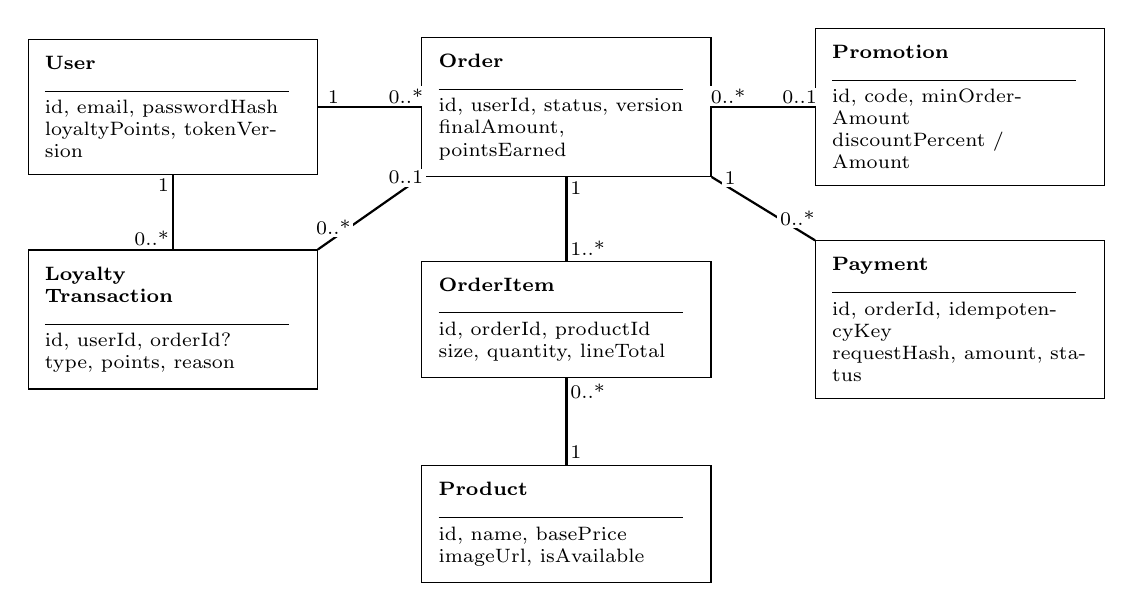
\begin{tikzpicture}[
  cls/.style={draw,rectangle,align=left,text width=3.25cm,inner sep=6pt,font=\scriptsize},
  rel/.style={thick}, mult/.style={font=\scriptsize,fill=white,inner sep=1pt}]
  \node[cls] (user) at (0,0) {\textbf{User}\\\rule{3.1cm}{0.3pt}\\id, email, passwordHash\\loyaltyPoints, tokenVersion};
  \node[cls] (order) at (5,0) {\textbf{Order}\\\rule{3.1cm}{0.3pt}\\id, userId, status, version\\finalAmount, pointsEarned};
  \node[cls] (promo) at (10,0) {\textbf{Promotion}\\\rule{3.1cm}{0.3pt}\\id, code, minOrderAmount\\discountPercent / Amount};
  \node[cls] (loyalty) at (0,-2.7) {\textbf{Loyalty}\\\textbf{Transaction}\\\rule{3.1cm}{0.3pt}\\id, userId, orderId?\\type, points, reason};
  \node[cls] (item) at (5,-2.7) {\textbf{OrderItem}\\\rule{3.1cm}{0.3pt}\\id, orderId, productId\\size, quantity, lineTotal};
  \node[cls] (payment) at (10,-2.7) {\textbf{Payment}\\\rule{3.1cm}{0.3pt}\\id, orderId, idempotencyKey\\requestHash, amount, status};
  \node[cls] (product) at (5,-5.3) {\textbf{Product}\\\rule{3.1cm}{0.3pt}\\id, name, basePrice\\imageUrl, isAvailable};
  \draw[rel] (user) -- node[mult,pos=.15,above]{1} node[mult,pos=.85,above]{0..*} (order);
  \draw[rel] (order) -- node[mult,pos=.16,above]{0..*} node[mult,pos=.85,above]{0..1} (promo);
  \draw[rel] (user) -- node[mult,pos=.14,left]{1} node[mult,pos=.85,left]{0..*} (loyalty);
  \draw[rel] (order) -- node[mult,pos=.14,right]{1} node[mult,pos=.85,right]{1..*} (item);
  \draw[rel] (order.south east) -- node[mult,pos=.18,above]{1} node[mult,pos=.83,above]{0..*} (payment.north west);
  \draw[rel] (order.south west) -- node[mult,pos=.15,above]{0..1} node[mult,pos=.85,above]{0..*} (loyalty.north east);
  \draw[rel] (item) -- node[mult,pos=.15,right]{0..*} node[mult,pos=.85,right]{1} (product);
\end{tikzpicture}
\caption{Bảy lớp nghiệp vụ cốt lõi. Bội số 1..* dòng/đơn là quy tắc khi tạo đơn; khóa ngoại riêng lẻ không tự bảo đảm một đơn luôn có dòng. Các lớp phụ được mô tả trong bảng dữ liệu.}
\label{fig:domain-core}
\end{figure}

Các ràng buộc unique và khóa ngoại hỗ trợ tính toàn vẹn, nhưng không thay thế kiểm tra nghiệp vụ trong service. Ví dụ, một Order có nhiều Payment để thử lại sau lỗi; không thể đặt unique trên \texttt{Payment.orderId} để chống lặp vì sẽ mất khả năng này. Nguồn mô hình: \path{backend/prisma/schema.prisma}.

\subsection{Trạng thái đơn và tính nhất quán khi đặt đồng thời}

Luồng thành công là \texttt{PENDING} $\rightarrow$ \texttt{PAID} $\rightarrow$ \texttt{PREPARING} $\rightarrow$ \texttt{READY} $\rightarrow$ \texttt{COMPLETED}. Khi thanh toán lỗi, \texttt{PENDING} $\rightarrow$ \texttt{PAYMENT\_FAILED}; thử lại đi qua \texttt{PAYMENT\_FAILED} $\rightarrow$ \texttt{PENDING}. Hủy được cho phép từ \texttt{PENDING}, \texttt{PAYMENT\_FAILED} hoặc \texttt{PAID}; \texttt{COMPLETED} và \texttt{CANCELLED} là trạng thái kết thúc. Hàm \texttt{assertOrderTransition} chỉ cho các cạnh đã khai báo; cập nhật trạng thái còn phải khớp trạng thái và version hiện tại. Các bước pha chế thể hiện state machine Task 10; giao diện nhân viên/quản trị là phần mở rộng so với MVP khách hàng.

Khi tạo đơn, backend đọc sản phẩm và bảng giá theo size, tính lại topping, kiểm tra mã khuyến mãi theo ngày hiệu lực/giá trị đơn, rồi áp dụng điểm được phép dùng. Điểm sử dụng phải là bội số của 10; 10 điểm tương ứng 1.000 VNĐ. Backend giảm số dư bằng cập nhật có điều kiện đủ điểm, không dựa vào số dư UI đã tải trước đó.

Tồn kho hiện được kiểm soát theo \emph{nguyên liệu và công thức}: tổng lượng nguyên liệu cần cho từng sản phẩm--size được nhân số ly và cộng gộp. Trong transaction mức cô lập Serializable, mỗi nguyên liệu được trừ bằng cập nhật có điều kiện \texttt{id + version + stock >= lượng cần}; thành công tăng version. Không đủ kho, thiếu công thức hoặc xung đột cập nhật làm transaction thất bại, không để lại đơn/tồn/điểm ở trạng thái dở dang. Lỗi xung đột Serializable của Prisma (P2034) được đổi thành HTTP 409 để khách kiểm tra và thử lại; service không tự lặp vô hạn. Topping được trừ tồn riêng bằng điều kiện đủ số lượng. Trường \texttt{Product.stock} vẫn có trong schema nhưng không phải nguồn kiểm soát tồn trong luồng tạo đơn này.

Lượng nguyên liệu đã giữ được lưu ở \texttt{OrderIngredient}; hủy đơn hoàn theo dữ liệu chốt đó, tránh công thức bị sửa sau khi đặt làm hoàn sai kho. Hủy còn hoàn topping và điểm đã dùng; nếu đơn đã trả tiền thì đảo điểm được cộng và đánh dấu \texttt{MANUAL\_REQUIRED} cho hoàn tiền thủ công, không giả định có hoàn tiền tự động qua cổng. Tác vụ mỗi phút tìm đơn \texttt{PENDING} được tạo quá 15 phút để hủy qua cùng nghiệp vụ. Bộ quét hiện chỉ xét \texttt{PENDING}, không tự giải phóng mọi đơn \texttt{PAYMENT\_FAILED}; đây là giới hạn vận hành cần theo dõi.

Nguồn: \path{backend/src/modules/orders/order-state.ts} và \path{backend/src/modules/orders/orders.service.ts}.

\subsection{Thanh toán idempotent và chuỗi tương tác}

\texttt{POST /payments/zalopay} nhận \texttt{orderId}, phương thức Ví/Thẻ và header \texttt{Idempotency-Key} dài 1--255 ký tự. Số tiền lấy từ \texttt{Order.finalAmount}. Service lưu SHA-256 của nội dung yêu cầu (gồm nguồn thanh toán, đơn và phương thức). Cùng key, cùng chủ đơn và cùng nội dung trả lại kết quả cũ; cùng key nhưng nội dung khác trả 409. Ràng buộc unique trên key là lớp bảo vệ tại CSDL khi các yêu cầu đến đồng thời.

Trong transaction tạo giao dịch, backend khóa dòng đơn bằng \texttt{SELECT ... FOR UPDATE}, kiểm tra lại key sau khi chờ khóa, trạng thái đơn và lượt thanh toán đang xử lý/thành công. Service ghi Payment \texttt{PENDING} \emph{trước} khi gọi mạng để kết quả không xác định không thể mở thêm lượt thu tiền. Sau đó backend ký HMAC-SHA256 và gọi API create của ZaloPay Sandbox. Khi callback hoặc truy vấn xác nhận đúng mã giao dịch và số tiền, Payment chuyển \texttt{SUCCESS} và đơn chuyển \texttt{PAID} trong cùng transaction; điểm thưởng bằng $\lfloor\mathrm{finalAmount}/1000\rfloor$ được cộng và ghi sổ một lần. Khóa dòng, kiểm tra trạng thái, cập nhật có version và replay kết quả giúp lần gửi lặp không cộng điểm thêm.

\begin{figure}[htbp]
\centering
\begin{tikzpicture}[
  head/.style={draw,rounded corners,minimum height=.65cm,align=center,font=\small,inner sep=4pt},
  msg/.style={-{Latex[length=1.7mm]},thick},
  ret/.style={-{Latex[length=1.7mm]},dashed},
  lab/.style={font=\scriptsize,align=center,fill=white,inner sep=1pt}]
  \node[head] at (0,0) {Khách};
  \node[head] at (2.1,0) {Next.js UI};
  \node[head] at (5.4,0) {NestJS API};
  \node[head] at (9.1,0) {PostgreSQL};
  \node[head] at (12.1,0) {ZaloPay};
  \foreach \x in {0,2.1,5.4,9.1,12.1} \draw[dashed,gray] (\x,-.4) -- (\x,-9.35);
  \draw[msg] (0,-.95) -- node[lab,above]{Xác nhận món} (2.1,-.95);
  \draw[msg] (2.1,-1.6) -- node[lab,above]{POST /orders + JWT} (5.4,-1.6);
  \draw[msg] (5.4,-2.35) -- node[lab,above]{Serializable: giá, kho, điểm; tạo đơn} (9.1,-2.35);
  \draw[ret] (9.1,-2.95) -- node[lab,above]{Commit: PENDING} (5.4,-2.95);
  \draw[ret] (5.4,-3.55) -- node[lab,above]{Mã đơn, thành tiền} (2.1,-3.55);
  \draw[msg] (0,-4.2) -- node[lab,above]{Chọn Ví / Thẻ} (2.1,-4.2);
  \draw[msg] (2.1,-4.9) -- node[lab,above]{POST /payments/zalopay\\JWT + Idempotency-Key} (5.4,-4.9);
  \draw[msg] (5.4,-5.7) -- node[lab,above]{BEGIN; khóa đơn; tạo Payment PENDING} (9.1,-5.7);
  \draw[msg] (5.4,-6.45) -- node[lab,above]{create: HMAC + app\_trans\_id} (12.1,-6.45);
  \draw[ret] (12.1,-7.05) -- node[lab,above]{order\_url hoặc lỗi} (5.4,-7.05);
  \draw[msg] (5.4,-7.8) -- node[lab,above]{callback/query xác nhận; PAID + điểm; COMMIT} (9.1,-7.8);
  \draw[ret] (5.4,-8.5) -- node[lab,above]{Kết quả đã lưu} (2.1,-8.5);
  \draw[ret] (2.1,-9.1) -- node[lab,above]{Hiển thị kết quả} (0,-9.1);
\end{tikzpicture}
\caption{Chuỗi checkout và thanh toán ZaloPay Sandbox. Nhánh replay trả kết quả đã lưu; nhánh lỗi giao dịch rollback và trả lỗi, không được vẽ lại để giữ sơ đồ dễ đọc.}
\label{fig:checkout-sequence}
\end{figure}

UI lưu key của lần thử trong sessionStorage để có thể dùng lại khi mất phản hồi; khi thành công mới kết thúc đơn chờ và cập nhật giỏ. Khi thất bại, giỏ được giữ để khách thử lại. Tuy nhiên, idempotency của Payment không đồng nghĩa \texttt{POST /orders} có idempotency key: frontend có logic đối chiếu đơn chờ, còn khi kết nối bị ngắt cần kiểm tra lịch sử trước khi đặt lại.

\textbf{Giới hạn thanh toán:} ZaloPay Sandbox chỉ được bật khi \texttt{NODE\_ENV} là \texttt{development}/\texttt{test}, \texttt{ZALOPAY\_SANDBOX\_ENABLED=true} và có đủ \texttt{ZALOPAY\_APP\_ID}/\texttt{KEY1}/\texttt{KEY2}; môi trường khác bị từ chối. Kết quả không xác định (timeout, mã lỗi truy vấn) giữ Payment \texttt{PENDING} và trả 503, không tự kết luận thất bại. Đây là luồng thử nghiệm có kiểm chứng chữ ký, không chứng minh khả năng thu tiền production.

Nguồn: \path{backend/src/modules/payments/zalopay-sandbox.service.ts}, \path{backend/src/modules/payments/zalopay-sandbox.gateway.ts}, \path{backend/src/modules/payments/zalopay-sandbox.controller.ts}, \path{frontend/src/app/orders/[id]/payment/page.tsx} và \path{frontend/src/lib/pending-order.ts}.

\subsection{Triển khai cục bộ và dữ liệu khởi tạo}

Docker Compose định nghĩa ba service trên máy phát triển: frontend, backend và postgres. Trình duyệt truy cập frontend ở cổng 3000 và gọi API công khai ở cổng 4000. Backend kết nối tới hostname nội bộ \texttt{postgres:5432}; cổng PostgreSQL xuất ra máy host mặc định là 5433 và có thể đổi bằng \texttt{POSTGRES\_PORT}. URL API của frontend được đưa vào lúc build bằng \texttt{NEXT\_PUBLIC\_API\_URL}, nên giá trị localhost chỉ phù hợp với trình duyệt chạy trên máy demo.

\begin{figure}[htbp]
\centering
\begin{tikzpicture}[
  box/.style={draw,rounded corners,text width=3.2cm,minimum height=1.05cm,align=center,font=\small},
  flow/.style={-{Latex[length=2mm]},thick},
  lab/.style={font=\scriptsize,align=center,fill=white,inner sep=2pt}]
  \node[box] (browser) at (0,0) {Trình duyệt\\máy phát triển};
  \node[box] (fe) at (5,0) {frontend\\Next.js :3000};
  \node[box] (be) at (5,-2.5) {backend\\NestJS :4000};
  \node[box] (db) at (10,-2.5) {postgres\\PostgreSQL 16 :5432};
  \node[box] (disk) at (10,-4.7) {Volume\\\texttt{brewlite\_}\\\texttt{postgres\_data}};
  \node[draw,dashed,rounded corners,fit=(fe)(be)(db)(disk),inner sep=10pt,label={[font=\small]above:Docker Compose cục bộ}] {};
  \draw[flow] (browser) -- node[lab,above]{localhost:3000} (fe);
  \draw[flow] (browser.south) |- node[lab,pos=.72,above]{REST: localhost:4000/api/v1} (be.west);
  \draw[flow] (be) -- node[lab,above]{DATABASE\_URL\\postgres:5432} (db);
  \draw[flow] (db) -- node[lab,right]{lưu bền} (disk);
\end{tikzpicture}
\caption{Sơ đồ triển khai local. Host có thể truy cập DB qua 5433:5432; ZaloPay là dịch vụ ngoài nên không có container hay cổng riêng.}
\label{fig:local-deployment}
\end{figure}

Hai Dockerfile dùng Node 22 Alpine, cài phụ thuộc bằng \texttt{npm ci} và build ứng dụng. Backend sinh Prisma Client khi build; lúc container khởi động chạy \texttt{prisma migrate deploy} trước khi chạy NestJS. Backend chỉ khởi động sau khi PostgreSQL vượt healthcheck; frontend có phụ thuộc thứ tự vào backend, không có nghĩa mọi API đã được kiểm tra sẵn sàng.

Volume \texttt{brewlite\_postgres\_data} giữ dữ liệu khi chạy \texttt{docker compose down} thông thường. Seed không tự chạy trong lệnh khởi động backend: \texttt{npm run prisma:seed} là thao tác riêng để nạp menu, công thức, nguyên liệu, ưu đãi và tài khoản demo. \textbf{Seed hiện xóa dữ liệu cũ trước khi tạo lại}, do đó chỉ dùng với CSDL local/test có thể đặt lại; không coi đây là thao tác nâng cấp dữ liệu vận hành. Migration cập nhật cấu trúc CSDL và seed tạo dữ liệu mẫu là hai việc khác nhau.

Đây là cấu hình chạy thử tại máy, không phải minh chứng đã triển khai production. Không suy ra từ Dockerfile rằng hệ thống đã có TLS, quản lý bí mật, sao lưu/khôi phục, nhiều replica hay CI/CD. Nguồn: \path{docker-compose.yml}, \path{backend/Dockerfile}, \path{frontend/Dockerfile}, \path{backend/prisma/seed.ts} và \path{README.md}.

\subsection{Lựa chọn công nghệ và đánh đổi}

\begin{itemize}[leftmargin=*,itemsep=4pt]
  \item \textbf{Next.js + TypeScript + Tailwind CSS:} phù hợp công nghệ bắt buộc và tổ chức trang theo App Router. React state/localStorage giúp giỏ nháp tồn tại sau khi tải lại trang với ít hạ tầng; đánh đổi là giỏ phụ thuộc trình duyệt, chưa được đồng bộ qua tài khoản và chưa sử dụng store Zustand/Context như gợi ý Task 5.
  \item \textbf{NestJS + Passport + class-validator:} module/controller/service và dependency injection tạo ranh giới nghiệp vụ rõ; DTO và guard dùng chung giảm lặp kiểm tra HTTP. Tách frontend/backend yêu cầu cấu hình URL và CORS nhất quán, đồng thời xử lý trạng thái lỗi mạng ở UI.
  \item \textbf{Prisma + PostgreSQL:} quan hệ và transaction phù hợp cập nhật đơn--kho--điểm cùng lúc. Prisma hỗ trợ schema/migration và truy vấn có kiểu; riêng khóa dòng thanh toán vẫn cần SQL \texttt{FOR UPDATE}. Serializable và optimistic locking ưu tiên nhất quán, đổi lại có thể trả 409 khi tranh chấp thay vì mọi yêu cầu đều thành công.
  \item \textbf{ZaloPay Sandbox + Compose:} cho phép trình diễn tạo giao dịch, callback, truy vấn, hủy và gửi lặp mà không dùng tiền thật. Đổi lại, cần cấu hình sandbox và URL callback HTTPS; kết quả không đại diện đầy đủ hợp đồng merchant production và CI không gọi mạng ZaloPay.
\end{itemize}

Các nhận định kiến trúc ở phần này dựa trên việc đọc mã nguồn và cấu hình. Mục tiêu API dưới 500 ms trong đề là tiêu chí cần đo bằng dữ liệu mẫu; phần này không khẳng định đã đạt hiệu năng, đã chạy toàn bộ kiểm thử hay đã triển khai thực tế khi chưa có kết quả tương ứng.
